%%%%%%%%%%%%%%%%%%%%%%%%%%%%%%%%%%%%%%%%%%%%%%%%%%%%%%%%%%%%%%%%%%%%%%
%%
%% This LaTeX file typesets the User's Guide for fbe_tez.sty.
%%
%%%%%%%%%%%%%%%%%%%%%%%%%%%%%%%%%%%%%%%%%%%%%%%%%%%%%%%%%%%%%%%%%%%%%%
%%
%% COPYRIGHT 1999, 2001, 2003 by
%% Feza Kerestecioglu <kerestec@boun.edu.tr>
%%
%% Copying of part or all of any file in the fbe_tez package is
%% allowed under the following conditions only:
%% (1) You may freely distribute unchanged copies of the files. Please
%%     include the documentation when you do so.
%% (2) You may modify a renamed copy of any file, but only for your
%%     personal use.
%% (3) You may copy fragments from the files, for personal use only
%%     and as long as credit is given where credit is due.
%%
%% You are NOT ALLOWED to take money for the distribution or use of
%% these files or modified versions or fragments thereof.
%%
%%%%%%%%%%%%%%%%%%%%%%%%%%%%%%%%%%%%%%%%%%%%%%%%%%%%%%%%%%%%%%%%%%%%%%
%

\documentclass[12pt]{article}
\usepackage{float}
%\usepackage[bottom]{footmisc}
\usepackage{cite}
\usepackage{graphicx}
\usepackage{longtable}
\graphicspath{{figures/}} % Graphics will be here

%
% Pagestyle
%
\oddsidemargin9.6mm
\evensidemargin9.6mm
\topmargin-1cm
\headheight20pt
\textwidth155mm
\textheight232mm
\pagestyle{myheadings}
%
% Macros
%
\newcommand\fbe{{\tt fbe\_tez}}
\newcommand\report{{\tt report}}
\newcommand{\bq}{\begin{quotation}\noindent}
\newcommand{\eq}{\end{quotation}}
\renewcommand{\arg}[1]{$\langle\mbox{\it #1}\rangle$}
%
% Title declarations
%

\title{{\Huge CmpE 443 Final Project Design Document} \\ Group Name: Tezla  }
\author{Members \\ Abdurrahman DILMAC (Team Leader) \\ Ahmet Semih ARI\\ Ramazan ARSLAN\\ Yunus Emre DEMIRCI}
\date{December 12, 2018 \\ Version 1.00}
%
\begin{document}
\maketitle
\tableofcontents
\newpage
\section{System Level Structural Diagram (Block Diagram)}

This is where system level structural diagram will be put. Do not forget to describe functionality of the components in the scope of the given problem.

\newpage
\section{Sequence Diagram}

Sequence Diagram would be here. You should show the high level relationships between modules clearly (you do not need to give details such as variable names and function names). The relationship between the hardwares and the software must be demonstrated in this diagram.  Explain each module as in your labs. Example Sequence Diagram for Lab 7 is provided below Figure:
\begin{figure}[htbp]
\begin{center}
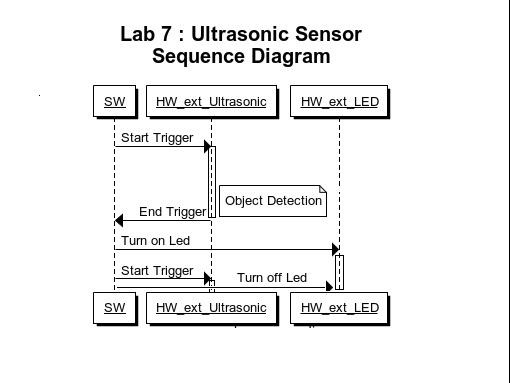
\includegraphics[width=1\columnwidth]{seqDiagram1.jpg}
\end{center}
\caption{Sample Sequence Diagram.}
\vskip\baselineskip % Leave a vertical skip below the figure
\label{fig:sample}
\end{figure}
\newpage
\section{LED Connections}

All the components which are controlled via LPC4088 should be connected to the board. Therefore, you should determine the pins and their functionalities. Draw the described table in the term project interim report description document. After you determine the all the pins, draw the circuit schematic for the LED circuits.
\newpage
\section{Motor - Speed Sensor Connection}

You should determine the pins of sensors and their functionalities.Draw a table which shows the pins and their functionalities as described in the project description document.
\newpage
\section{Motor - Driver Connection}
Here is an example figure for you to use the LaTeX format. \\ \\
\begin{figure}[htbp]
\begin{center}
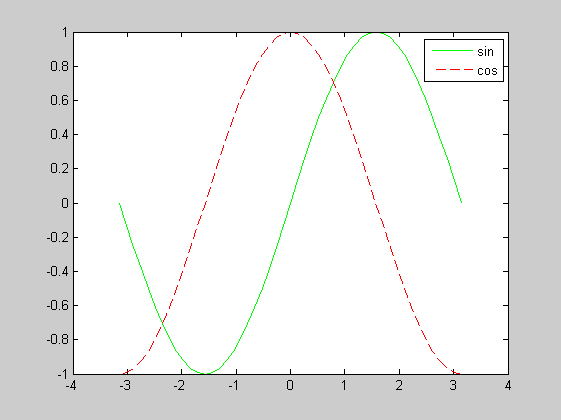
\includegraphics[width=0.5\columnwidth]{sample_figure.png}
\end{center}
\caption{Sin and
Cosine.}
\vskip\baselineskip % Leave a vertical skip below the figure
\label{fig:sample}
\end{figure}
\newpage
\section{Driver - Board Connection}

Here is an example table for you to use the LaTeX format.\\ \\



\begin {table}[H]
\begin{tabular}{|p{1in}|p{1in}|p{1in}|p{1in}|p{1in}|} \hline 
\textbf{Algorithm} & \textbf{Feature 1} & \textbf{Feature 2} & \textbf{ Feature 3} & \textbf{Feature n} \\ 
\hline 
\textbf{Alg 1} & 1 & \textbf{2} & \textbf{23} & \textbf{68.7\%} \\ \hline 
\textbf{Alg 2} & \textbf{9} & \textbf{2} & \textbf{37} & \textbf{75.68\%} \\ \hline 
\textbf{Alg 3} & \textbf{10} & \textbf{3} & \textbf{51} & \textbf{96.34\%} \\ \hline 
\end{tabular}
\caption {Should be a caption}
\end {table}


\end{document}
%
% End of fbeman.tex
